\documentclass[ms]{agutexSI2019}

\usepackage{graphicx}
\usepackage{booktabs}
% agutexSI2019.cls's \endtable tests \iflandscapefigortab, but the class only defines
% \iflandscapetaborfig (a class typo); supply the missing conditional (false = normal table).
\newif\iflandscapefigortab
\def\journalname{Journal of Advances in Modeling Earth Systems}

\begin{document}

\title{Supporting Information for ``Controllable Probabilistic Forecasting with Stochastic Decomposition Layers''}

\authors{
John S. Schreck \affil{1},
William E. Chapman \affil{1},
Charlie Becker \affil{1},
David John Gagne II \affil{1},
Dhamma Kimpara \affil{1},
Nihanth Cherukuru \affil{1},
Judith Berner \affil{1},
Kirsten J. Mayer \affil{1},
Negin Sobhani \affil{1}
}

\affiliation{1}{NSF National Center for Atmospheric Research, Boulder, CO, USA}

\noindent\textbf{Contents of this file}
\begin{enumerate}
\item Figures S1 to S3
\item Table S1
\end{enumerate}

\noindent\textbf{Introduction}

This Supporting Information provides the per-layer latent scaling analysis (Figures~S1--S2), the noise-scale selection sweep (Figure~S3), and the retrained design-choice ablations (Table~S1). Figures S1--S2 give the analysis of the main text's Figure~6 for two additional fields of differing spectral character, 700\,hPa specific humidity (Figure~S1) and mean sea-level pressure (Figure~S2). Both are computed with the identical protocol as the main-text figure: anomalies of ensemble member~0 relative to the deterministic forecast ($\beta=[0,0,0]$) for the Winter Storm Izzy case, valid January 17, 2022 at 18:00 UTC (108\,h lead time), with one per-scale gain varied across $[-3,3]$ per column while the remaining gains are held at unity. For all three fields examined (Z500 in the main text, Q700 and MSLP here), anomaly amplitude and spatial extent scale with $|\beta|$ at each injection site with consistent sign structure across the $\beta$ ladder, confirming that the per-layer interpretation of the main-text figure is not specific to the smoothness of geopotential.

\begin{figure}
\centering
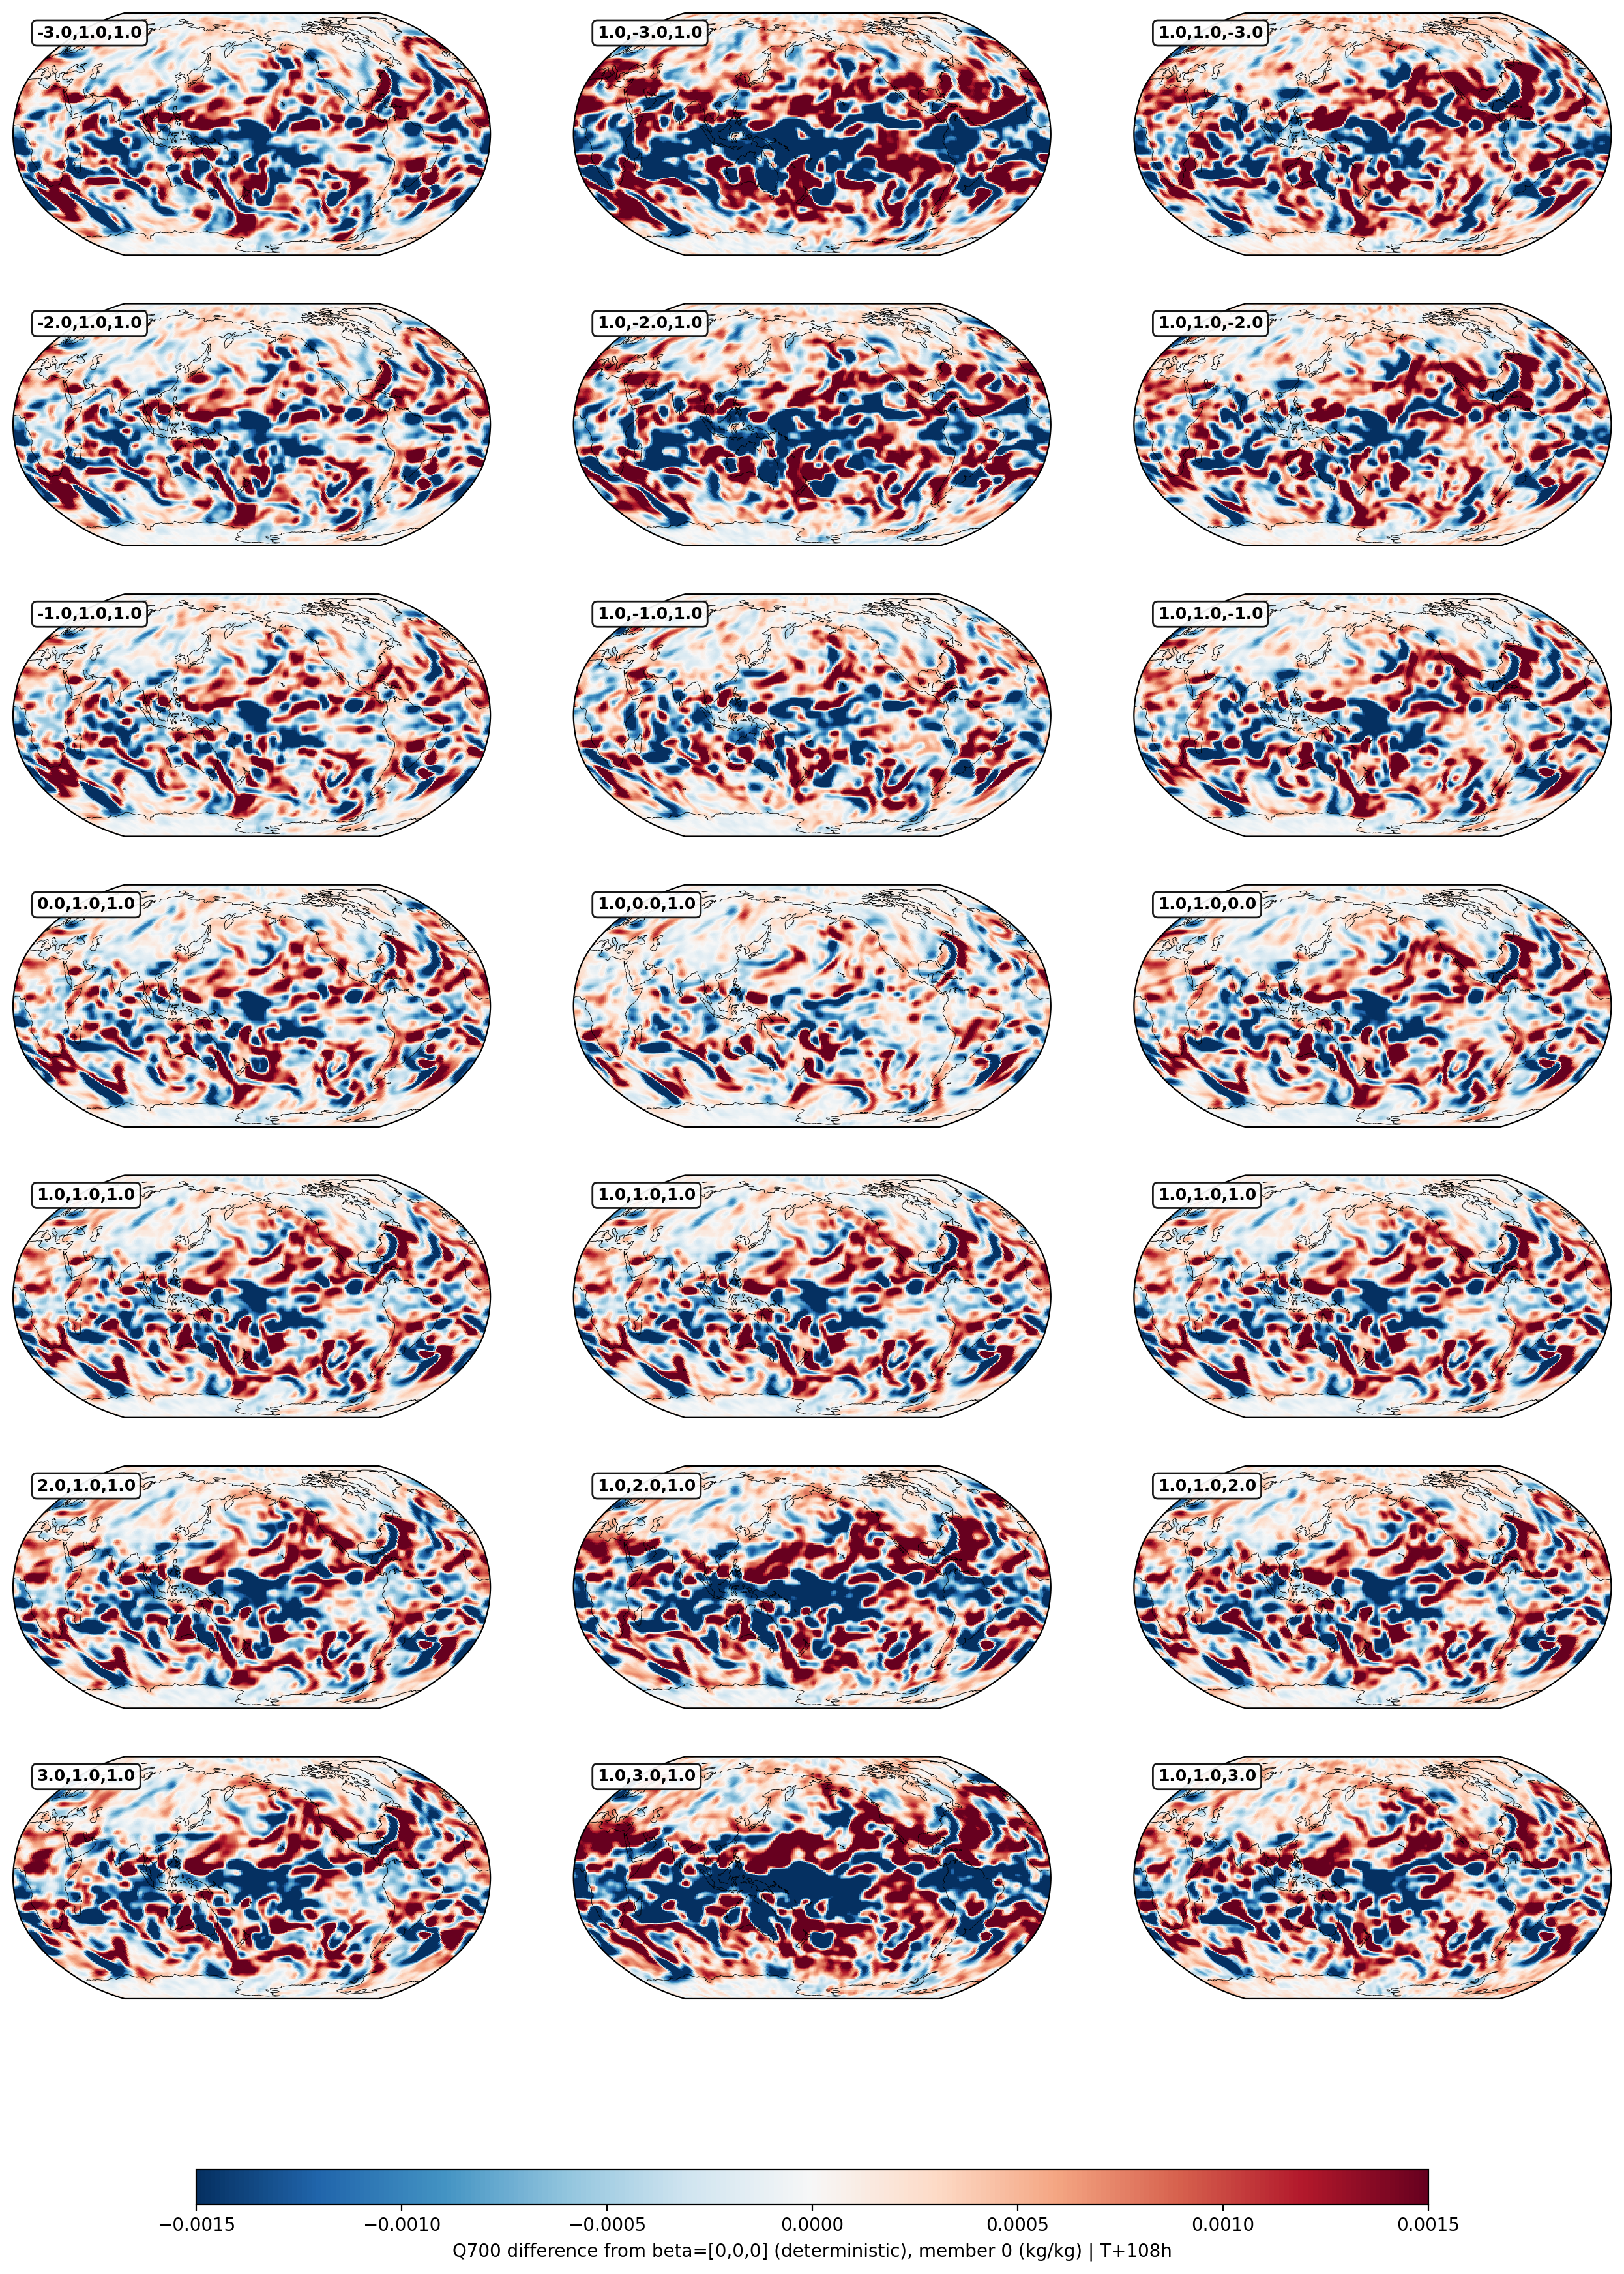
\includegraphics[width=\textwidth]{figure6_beta0ref_Q700.png}
\caption{As the main text's Figure~6, for 700\,hPa specific humidity: Q700 anomalies of member~0 from the deterministic forecast ($\beta=[0,0,0]$) under single-parameter variation of $\beta_1$ (left column), $\beta_2$ (center), and $\beta_3$ (right) across $[-3,3]$, remaining gains at unity. Valid 2022-01-17 18:00 UTC (108\,h lead).}
\label{fig:s1}
\end{figure}

\begin{figure}
\centering
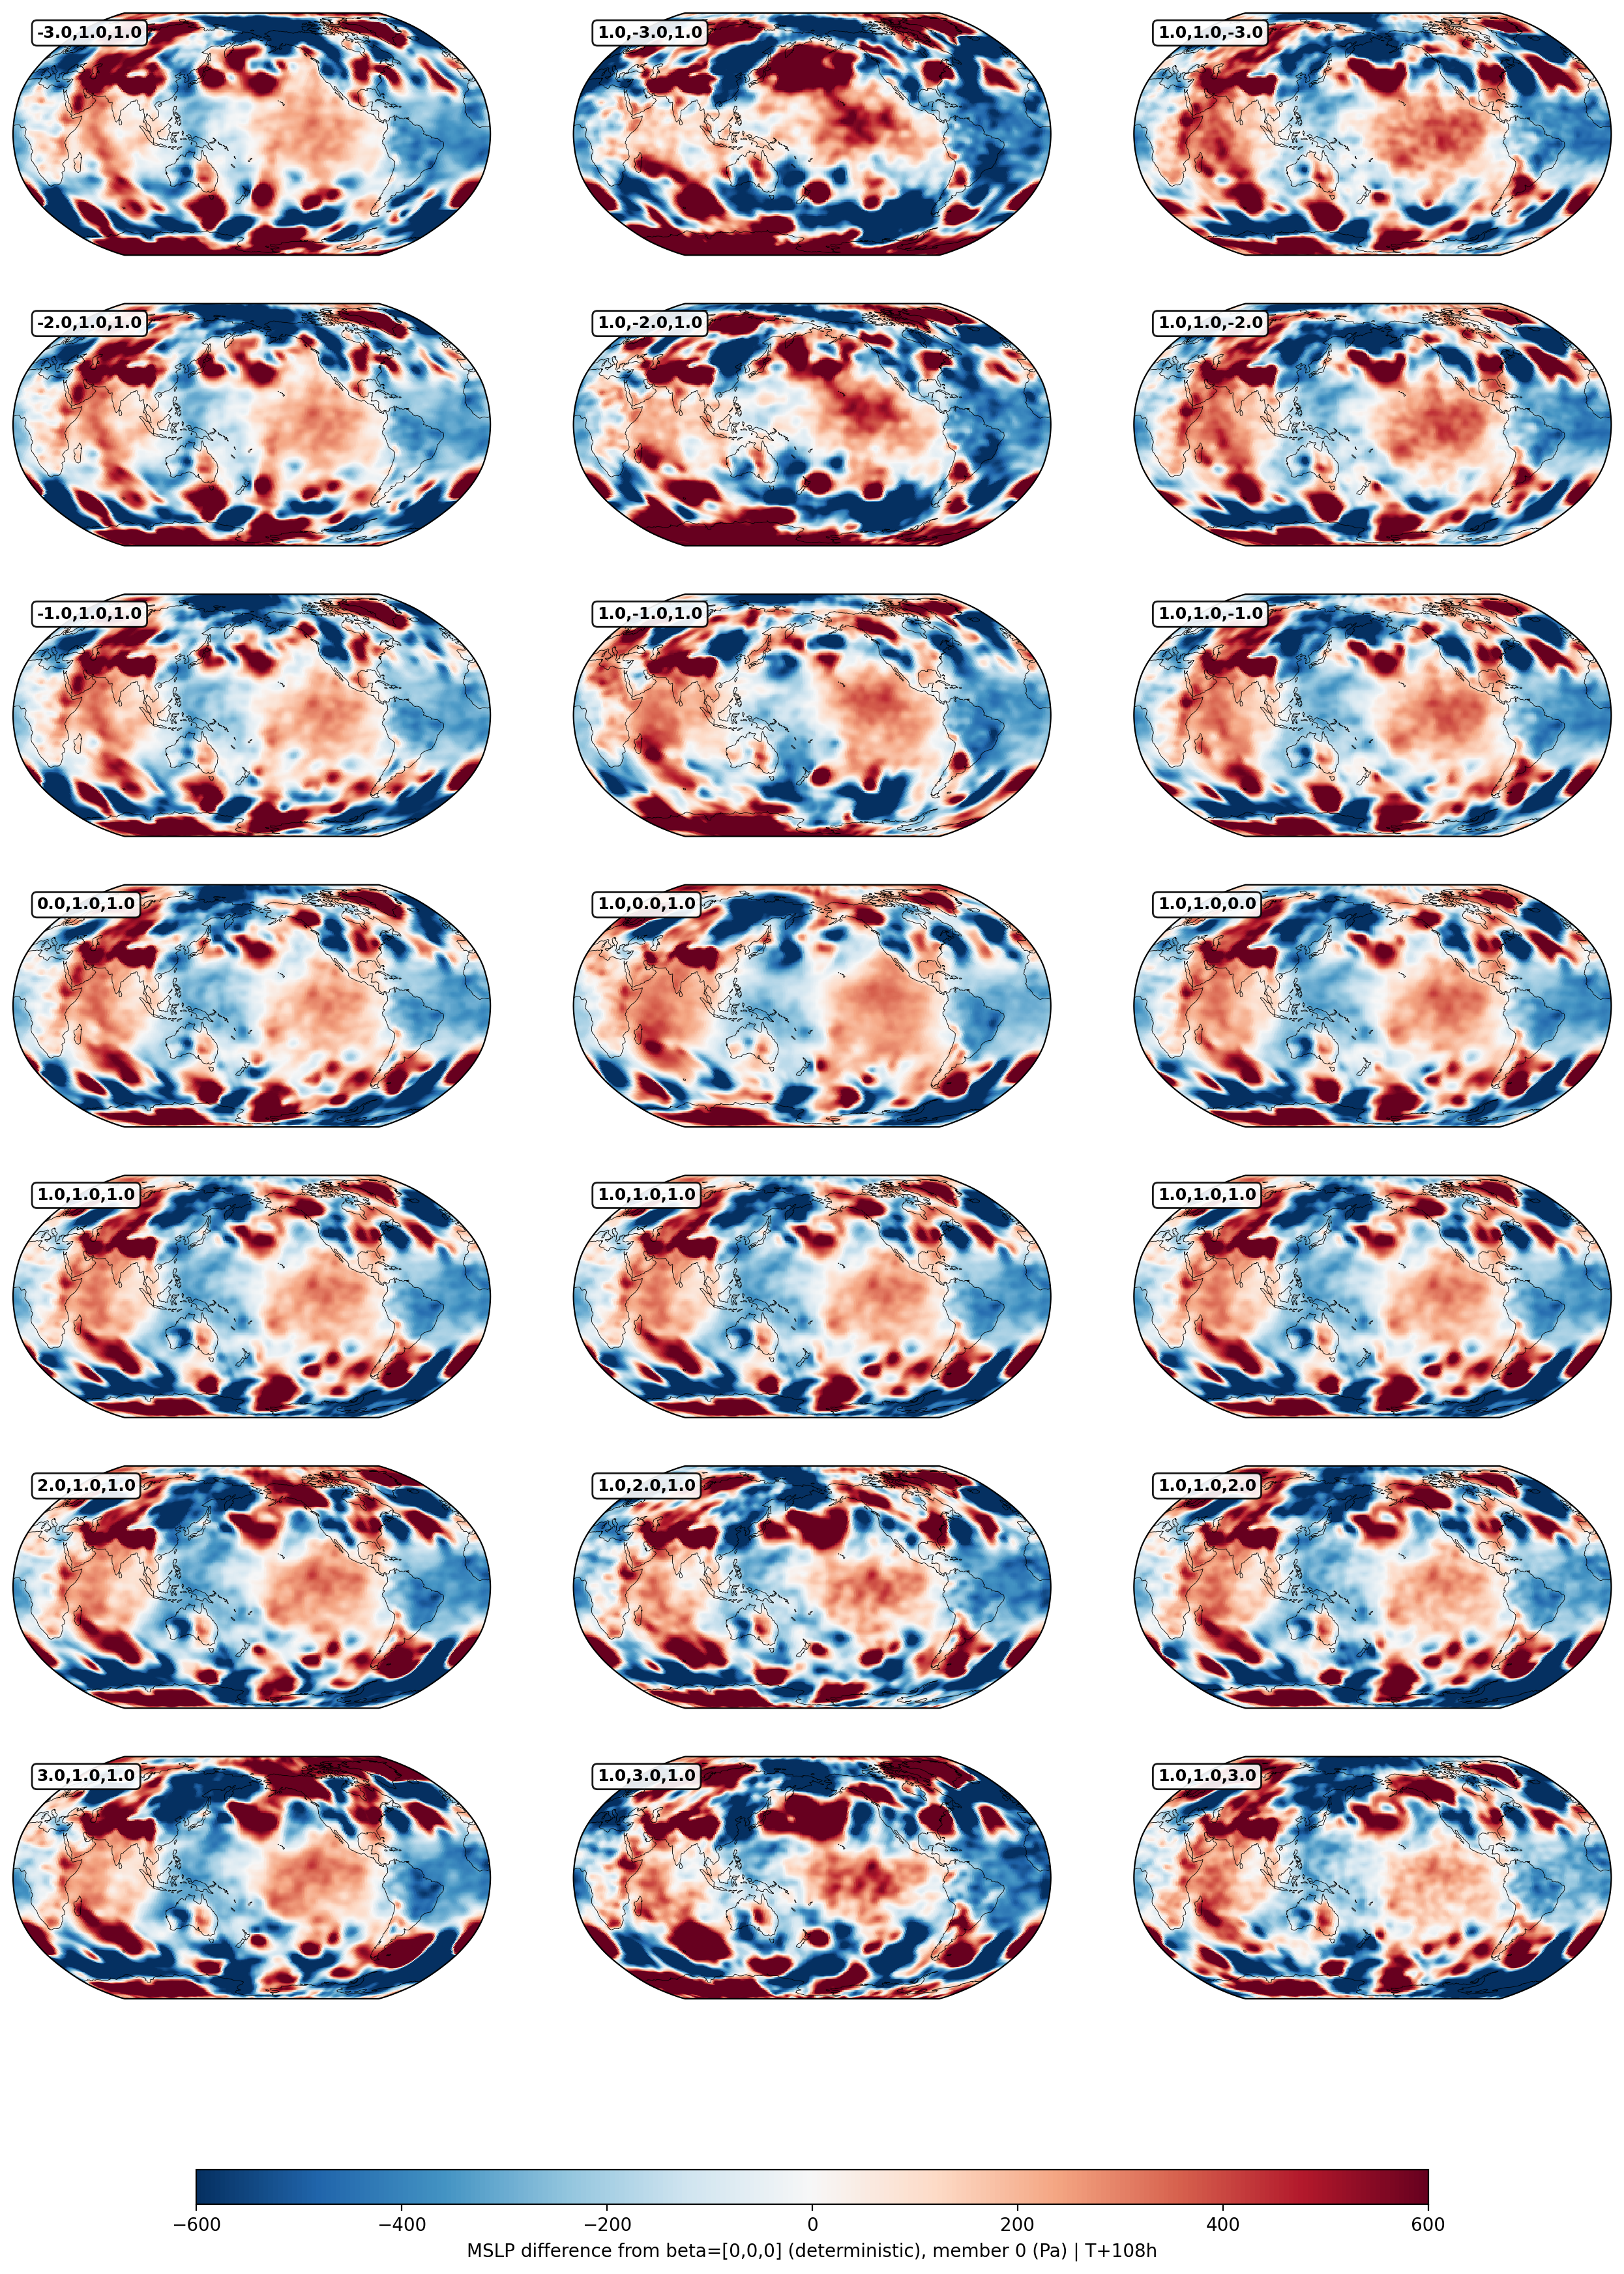
\includegraphics[width=\textwidth]{figure6_beta0ref_MSLP.png}
\caption{As Figure~S1, for mean sea-level pressure.}
\label{fig:s2}
\end{figure}

\begin{figure}
\centering
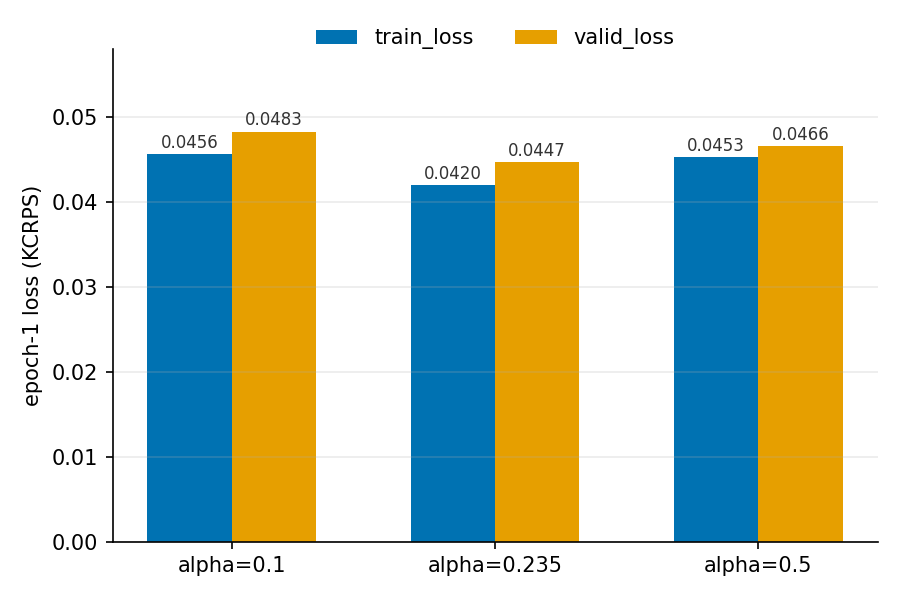
\includegraphics[width=0.85\textwidth]{alpha_sweep.png}
\caption{One-epoch sweep of the fixed noise-scaling parameter $\sigma_0 \in \{0.10, 0.235, 0.50\}$ used to select the value employed in the main text. Bars show training and validation loss after one epoch of fine-tuning from the deterministic base under otherwise identical configuration. $\sigma_0 = 0.235$ attains the lowest loss on both, roughly 7--8\% below either alternative, consistent with the minimize-initial-loss selection criterion described in Section~2.3. Because the injected perturbation is linear in $\sigma_0$ and in the learned components, $\sigma_0$ affects only the initialization scale and is held fixed thereafter.}
\label{fig:s3}
\end{figure}

% The class's table-float caption machinery misplaces the caption and emits a stray duplicate
% header (agutexSI2019.cls bug, incl. the undefined \iflandscapefigortab conditional in \endtable),
% so this single table is set as plain text: bold heading + caption paragraph + centered tabular.
\vspace{1em}
\noindent{\bf Table S1.} {\small Retrained design-choice ablations: percent difference from the published SDL model, averaged across Z500, T500, U500, V500, and Q500, from 20-member ensembles over 12 monthly 2022 00Z initializations (the first of each month) at three lead times. Positive RMSE/CRPS means worse than the published model. Negative Spread/SSR means less dispersive. Percent differences are insensitive to the latitude-weight normalization convention used in scoring. The reproducibility control refits the published configuration from the same deterministic base checkpoint with the identical loss configuration, seed, and 20-epoch schedule. Its rows set the run-to-run variability floor (roughly 1--4\%) against which the other variants should be read. Encoder-decoder injection and frozen backbone were trained under that same published configuration. The afCRPS pair is a matched pair of fine-tunes from a separate configuration lineage (a different seed) that is internally identical except for the correlated-noise flag, so the correlated-versus-independent comparison is clean within the pair but its rows are not directly comparable to the rows above. The same lineage applies to the frozen~$+$~correlated run, which additionally confounds the two flags and is included only to show that its degradation tracks the frozen backbone's, implicating the freeze rather than the correlation.}

\begin{center}
\small
\begin{tabular}{llrrrr}
\toprule
\textbf{Variant} & \textbf{Lead} & \textbf{RMSE} & \textbf{Spread} & \textbf{SSR} & \textbf{CRPS} \\
\midrule
Reproducibility control & 24\,h & $+0.4$ & $-1.2$ & $-1.7$ & $+0.8$ \\
 & 120\,h & $+1.9$ & $-2.1$ & $-3.9$ & $+2.7$ \\
 & 240\,h & $+1.2$ & $-1.5$ & $-2.6$ & $+2.1$ \\
\midrule
Encoder-decoder injection & 24\,h & $+0.4$ & $-3.8$ & $-4.2$ & $+1.3$ \\
 & 120\,h & $+1.2$ & $-3.8$ & $-5.0$ & $+2.5$ \\
 & 240\,h & $+0.4$ & $-2.9$ & $-3.3$ & $+1.7$ \\
\midrule
Frozen backbone & 24\,h & $+3.6$ & $-9.5$ & $-12.8$ & $+6.6$ \\
 & 120\,h & $+3.8$ & $-16.8$ & $-19.8$ & $+9.2$ \\
 & 240\,h & $+2.1$ & $-7.5$ & $-9.5$ & $+5.1$ \\
\midrule
afCRPS pair, independent & 24\,h & $+0.1$ & $-0.8$ & $-0.9$ & $+0.3$ \\
 & 120\,h & $+1.2$ & $-1.5$ & $-2.5$ & $+1.8$ \\
 & 240\,h & $+0.5$ & $-0.5$ & $-0.9$ & $+0.7$ \\
afCRPS pair, correlated & 24\,h & $+0.2$ & $-2.3$ & $-2.5$ & $+0.7$ \\
 & 120\,h & $+1.7$ & $-1.9$ & $-3.5$ & $+2.6$ \\
 & 240\,h & $-0.2$ & $-0.4$ & $-0.4$ & $+0.1$ \\
\midrule
Frozen $+$ correlated & 24\,h & $+4.3$ & $-10.4$ & $-14.3$ & $+7.7$ \\
 & 120\,h & $+4.1$ & $-15.6$ & $-18.9$ & $+9.6$ \\
 & 240\,h & $+1.5$ & $-7.2$ & $-8.7$ & $+3.9$ \\
\bottomrule
\end{tabular}
\end{center}

\end{document}
